%% abtex2-modelo-artigo.tex, v-1.9.7 laurocesar
%% Copyright 2012-2018 by abnTeX2 group at http://www.abntex.net.br/
%%
%% This work may be distributed and/or modified under the
%% conditions of the LaTeX Project Public License, either version 1.3
%% of this license or (at your option) any later version.
%% The latest version of this license is in
%%   http://www.latex-project.org/lppl.txt
%% and version 1.3 or later is part of all distributions of LaTeX
%% version 2005/12/01 or later.
%%
%% This work has the LPPL maintenance status `maintained'.
%%
%% The Current Maintainer of this work is the abnTeX2 team, led
%% by Lauro César Araujo. Further information are available on
%% http://www.abntex.net.br/
%%
%% This work consists of the files abntex2-modelo-artigo.tex and
%% abntex2-modelo-references.bib
%%

% ------------------------------------------------------------------------
% ------------------------------------------------------------------------
% abnTeX2: Modelo de Artigo Acadêmico em conformidade com
% ABNT NBR 6022:2018: Informação e documentação - Artigo em publicação
% periódica científica - Apresentação
% ------------------------------------------------------------------------
% ------------------------------------------------------------------------

\documentclass[
	% -- opções da classe memoir --
	article,			% indica que é um artigo acadêmico
	11pt,				% tamanho da fonte
	oneside,			% para impressão apenas no recto. Oposto a twoside
	a4paper,			% tamanho do papel.
	% -- opções da classe abntex2 --
	%chapter=TITLE,		% títulos de capítulos convertidos em letras maiúsculas
	%section=TITLE,		% títulos de seções convertidos em letras maiúsculas
	%subsection=TITLE,	% títulos de subseções convertidos em letras maiúsculas
	%subsubsection=TITLE % títulos de subsubseções convertidos em letras maiúsculas
	% -- opções do pacote babel --
	english,			% idioma adicional para hifenização
	brazil,				% o último idioma é o principal do documento
	sumario=tradicional
	]{abntex2}


% ---
% PACOTES
% ---

% ---
% Pacotes fundamentais
% ---
\usepackage{lmodern}			% Usa a fonte Latin Modern
\usepackage[T1]{fontenc}		% Selecao de codigos de fonte.
\usepackage[utf8]{inputenc}		% Codificacao do documento (conversão automática dos acentos)
\usepackage{indentfirst}		% Indenta o primeiro parágrafo de cada seção.
\usepackage{nomencl} 			% Lista de simbolos
\usepackage{color}				% Controle das cores
\usepackage{graphicx}			% Inclusão de gráficos
\usepackage{microtype} 			% para melhorias de justificação
% ---

% ---
% Pacotes adicionais, usados apenas no âmbito do Modelo Canônico do abnteX2
% ---
\usepackage{lipsum}				% para geração de dummy text
% ---


% ---
% Pacotes de citações
% ---
\usepackage[brazilian,hyperpageref]{backref}	 % Paginas com as citações na bibl
\usepackage[alf]{abntex2cite}	% Citações padrão ABNT
% ---

% ----
% Para o comentário de porções largas de código
% ----
\usepackage{comment}

% ---
% Configurações do pacote backref
% Usado sem a opção hyperpageref de backref
\renewcommand{\backrefpagesname}{Citado na(s) página(s):~}
% Texto padrão antes do número das páginas
\renewcommand{\backref}{}
% Define os textos da citação
\renewcommand*{\backrefalt}[4]{
	\ifcase #1 %
		Nenhuma citação no texto.%
	\or
		Citado na página #2.%
	\else
		Citado #1 vezes nas páginas #2.%
	\fi}%
% ---

% --- Informações de dados para CAPA e FOLHA DE ROSTO ---
\titulo{Trabalho da Disciplina CMC 103 -- Machine Learning}
\tituloestrangeiro{}

\autor{
Crisitano Gurgel de Castro\thanks{Inmetro, (21) 2679 9799, cgcastro at inmetro gov br}
}

\local{Duque de Caxias}
\data{\today}
% ---

% ---
% Configurações de aparência do PDF final

% alterando o aspecto da cor azul
\definecolor{blue}{RGB}{41,5,195}

% informações do PDF
\makeatletter
\hypersetup{
     	%pagebackref=true,
		%pdftitle={\@title},
		%pdfauthor={\@author},
    	%pdfsubject={Modelo de artigo científico com abnTeX2},
	   % pdfcreator={LaTeX with abnTeX2},
		%pdfkeywords={abnt}{latex}{abntex}{abntex2}{atigo científico},
		colorlinks=true,       		% false: boxed links; true: colored links
    	linkcolor=blue,          	% color of internal links
    	citecolor=blue,        		% color of links to bibliography
    	filecolor=magenta,      		% color of file links
		urlcolor=blue,
		bookmarksdepth=4
}
\makeatother
% ---

% ---
% compila o indice
% ---
\makeindex
% ---

% ---
% Altera as margens padrões
% ---
\setlrmarginsandblock{3cm}{3cm}{*}
\setulmarginsandblock{3cm}{3cm}{*}
\checkandfixthelayout
% ---

% ---
% Espaçamentos entre linhas e parágrafos
% ---

% O tamanho do parágrafo é dado por:
\setlength{\parindent}{1.3cm}

% Controle do espaçamento entre um parágrafo e outro:
\setlength{\parskip}{0.2cm}  % tente também \onelineskip

% Espaçamento simples
\SingleSpacing

% Definição do comando de questão
\newenvironment{comandoquestao}{\begin{citacao}\textbf{Comando:}}{\end{citacao}}


% ----
% Início do documento
% ----
\begin{document}

% Seleciona o idioma do documento (conforme pacotes do babel)
%\selectlanguage{english}
\selectlanguage{brazil}

% Retira espaço extra obsoleto entre as frases.
\frenchspacing

% ----------------------------------------------------------
% ELEMENTOS PRÉ-TEXTUAIS
% ----------------------------------------------------------

%---
%
% Se desejar escrever o artigo em duas colunas, descomente a linha abaixo
% e a linha com o texto ``FIM DE ARTIGO EM DUAS COLUNAS''.
% \twocolumn[    		% INICIO DE ARTIGO EM DUAS COLUNAS
%
%---

% página de titulo principal (obrigatório)
\maketitle


% titulo em outro idioma (opcional)



% resumo em português
\begin{comment}
\begin{resumoumacoluna}
   Conforme a ABNT NBR 6022:2018, o resumo no idioma do documento é elemento obrigatório.
   Constituído de uma sequência de frases concisas e objetivas e não de uma
   simples enumeração de tópicos, não ultrapassando 250 palavras, seguido, logo
   abaixo, das palavras representativas do conteúdo do trabalho, isto é,
   palavras-chave e/ou descritores, conforme a NBR 6028. (\ldots) As
   palavras-chave devem figurar logo abaixo do resumo, antecedidas da expressão
   Palavras-chave:, separadas entre si por ponto e finalizadas também por ponto.
   \vspace{\onelineskip}
   \noindent
   \textbf{Palavras-chave}: latex. abntex. editoração de texto.
  \end{resumoumacoluna}
\end{comment}



% resumo em inglês

% ]  				% FIM DE ARTIGO EM DUAS COLUNAS
% ---

\begin{center}\smaller
\textbf{Data de submissão}: 13 de novembro de 2024.

\begin{comment}
\textbf{Identificação e disponibilidade}: elemento opcional. Pode ser indicado
o endereço eletrônico, DOI, suportes e outras informações relativas ao acesso.
\end{comment}

\end{center}

% ----------------------------------------------------------
% ELEMENTOS TEXTUAIS
% ----------------------------------------------------------
\textual

% ----------------------------------------------------------
% Introdução
% ----------------------------------------------------------
\section{Introdução}

Na presente atividade, se propõe-se a conduzir uma análise de uma série de tarefas, cada uma focalizando diferentes parâmetros e hiperparâmetros associados às redes neurais artificiais. Com o objetivo principal de delinear a influência desses elementos técnicos sobre as propriedades comportamentais das redes neurais e obter elucidação de possíveis critérios e processos envolvidos na seleção desses parâmetros em aplicações práticas.

% ----------------------------------------------------------
% Seção de explicações
% ----------------------------------------------------------
\section{Tarefas Propostas}

Para as presentes tarefas, uma rede neural foi dada como exemplo. Tal rede é treinada para um conjunto de dados ${(x_i, y_i)}$ que refletem o comportamento de uma senóide $y_i = sen(x_i) + r_i$. Um ruído $r_i$ foi adicionado a cada medição de forma a refletir uma coleta de dados no mundo real com uma incerteza de medição associada

\subsection{Tarefa 1}

\begin{comandoquestao}
   Nesta tarefa, você explorará o impacto de diferentes funções de ativação no desempenho da rede neural. A função de ativação controla como os neurônios transformam os dados de entrada, e diferentes funções podem influenciar a capacidade de aprendizado da rede.
\end{comandoquestao}

A rede neural dada como exemplo utiliza a função Gelu como função de ativação nas camadas intermediárias. Vericamos o comportamento do erro de treinamento em relação ao número de épocas de treinamento (figura \ref{tarefa01:gelu:treinamento}), bem como a comparação dos dados previstos pela rede dados em relação aos dados de treinamento na figura \ref{tarefa01:gelu:predicoes}.

\begin{figure}[htb]
	\label{teste}
	\centering
	\begin{minipage}{0.45\textwidth}
	\centering
	\caption{Gelu: Treinamento} \label{tarefa01:gelu:treinamento}
	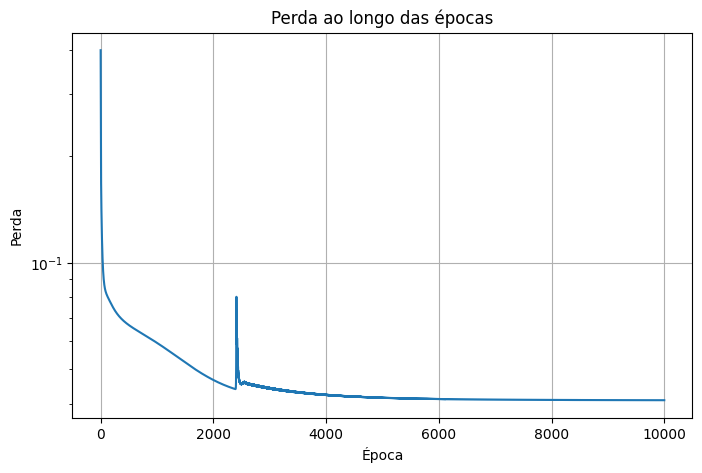
\includegraphics[width=\textwidth]{./0803_imgs/png-241111-212601400-7995113924505873963.png}
	%\legend{Fonte: Gerado peloComando da atividade}
	\end{minipage}
	\hfill
	\begin{minipage}{0.45\textwidth}
	\centering
	\caption{Gelu: predições} \label{tarefa01:gelu:predicoes}
	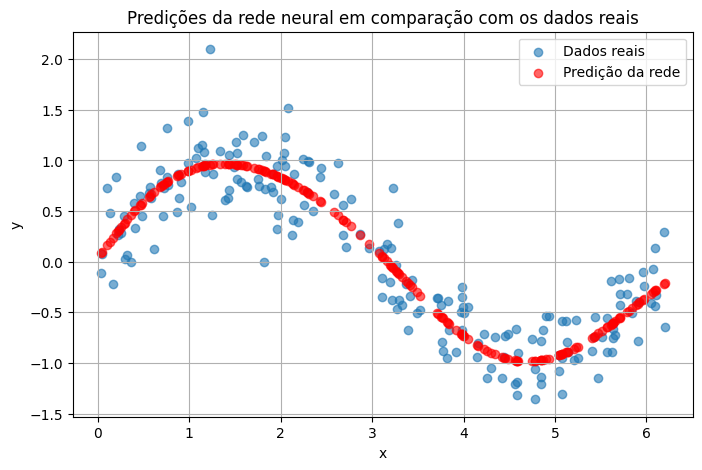
\includegraphics[width=\textwidth]{./0803_imgs/png-241111-212606975-12044568718402292765.png}
	%\legend{Fonte: \citeonline[p. 24]{araujo2012}}
	\end{minipage}
\end{figure}

Para a presente tarefa modificamos a função de ativação das camadas intermediárias para sigmóide, obtendo os resultados mostrados nas figuras


\begin{figure}[htb]
	\label{teste}
	\centering
	\begin{minipage}{0.45\textwidth}
	\centering
	\caption{Gelu: Treinamento} \label{tarefa01:gelu:treinamento}
	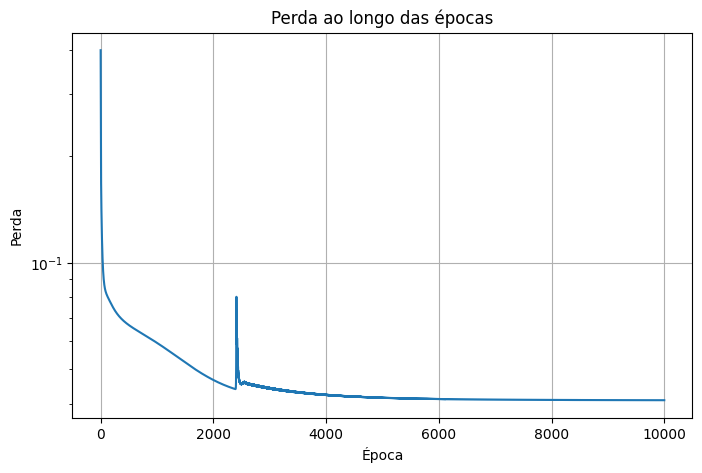
\includegraphics[width=\textwidth]{./0803_imgs/png-241111-212601400-7995113924505873963.png}
	%\legend{Fonte: Gerado peloComando da atividade}
	\end{minipage}
	\hfill
	\begin{minipage}{0.45\textwidth}
	\centering
	\caption{Gelu: predições} \label{tarefa01:gelu:predicoes}
	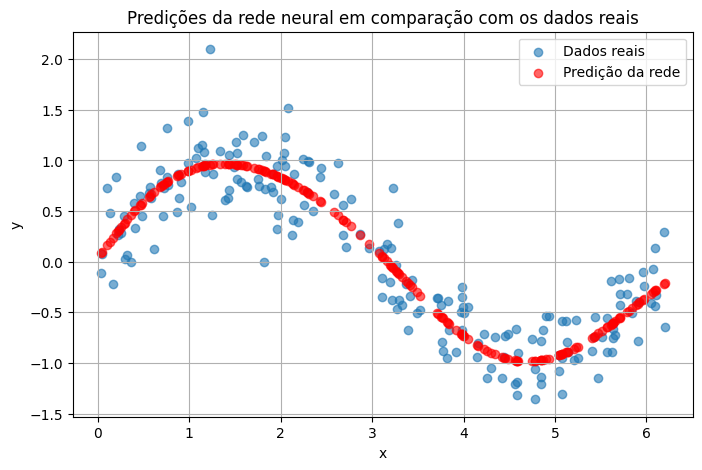
\includegraphics[width=\textwidth]{./0803_imgs/png-241111-212606975-12044568718402292765.png}
	%\legend{Fonte: \citeonline[p. 24]{araujo2012}}
	\end{minipage}
\end{figure}

%
\section{Consulte o manual da classe \textsf{abntex2}}

Consulte o manual da classe \textsf{abntex2} \cite{abntex2classe} para uma
referência completa das macros e ambientes disponíveis.

% ---
% Finaliza a parte no bookmark do PDF, para que se inicie o bookmark na raiz
% ---
\bookmarksetup{startatroot}%
% ---

% ---
% Conclusão
% ---
\section{Considerações finais}

\lipsum[1]

\begin{citacao}
\lipsum[2]
\end{citacao}

\lipsum[3]

% ----------------------------------------------------------
% ELEMENTOS PÓS-TEXTUAIS
% ----------------------------------------------------------
\postextual

% ----------------------------------------------------------
% Referências bibliográficas
% ----------------------------------------------------------
\bibliography{abntex2-modelo-references}

% ----------------------------------------------------------
% Glossário
% ----------------------------------------------------------
%
% Há diversas soluções prontas para glossário em LaTeX.
% Consulte o manual do abnTeX2 para obter sugestões.
%
%\glossary

% ----------------------------------------------------------
% Apêndices
% ----------------------------------------------------------

% ---
% Inicia os apêndices
% ---
\begin{apendicesenv}

% ----------------------------------------------------------
\chapter{Nullam elementum urna vel imperdiet sodales elit ipsum pharetra ligula
ac pretium ante justo a nulla curabitur tristique arcu eu metus}
% ----------------------------------------------------------
\lipsum[55-56]

\end{apendicesenv}
% ---

% ----------------------------------------------------------
% Anexos
% ----------------------------------------------------------
\cftinserthook{toc}{AAA}
% ---
% Inicia os anexos
% ---
%\anexos
\begin{anexosenv}

% ---
\chapter{Cras non urna sed feugiat cum sociis natoque penatibus et magnis dis
parturient montes nascetur ridiculus mus}
% ---

\lipsum[31]

\end{anexosenv}

% ----------------------------------------------------------
% Agradecimentos
% ----------------------------------------------------------
\section*{Agradecimentos}
Texto sucinto aprovado pelo periódico em que será publicado. Último
elemento pós-textual.



\end{document}
